\documentclass[justified]{tufte-handout}
\usepackage{braph2_tut}
%\geometry{showframe} % display margins for debugging page layout

\title{Getting Started}

\begin{document}

\maketitle

\begin{abstract}
\noindent
This tutorial provides a concise introduction to the BRAPH-2 software framework, which enables comprehensive analyses of brain connectivity using conventional graph theory, advanced multilayer network, and deep learning approaches. BRAPH-2 has been designed following an object-oriented paradigm and supports workflows involving structural, functional, and connectivity data derived from multimodal neuroimaging techniques (e.g., MRI, dMRI, fMRI). It offers a set of ready-made pipelines to compute graph measures, perform group-level comparisons, and apply classification or regression tasks with deep learning, all accessible via an intuitive graphical user interface (GUI) or through MATLAB scripts. BRAPH-2 also facilitates more advanced network neuroscience investigations by enabling the construction and analysis of multilayer graphs, permitting the user to probe how multiple types of data interact across layers (e.g., combining anatomical and functional information). To ensure reproducibility and expandability, BRAPH-2 integrates a ``lock in'' mechanism that saves and freezes data, parameters, and random seeds along the analysis pipeline. Moreover, developers can extend BRAPH-2 by adding new graph measures, neural network architectures, or analysis pipelines. In this tutorial, we outline the major steps for installing and running BRAPH-2, preparing datasets, creating and executing pipelines, and interpreting results, as well as point to developer resources for deeper customization.
\end{abstract}

\tableofcontents

\clearpage

\section{Introduction}

BRAPH-2 is an open-source MATLAB-based toolbox for brain connectivity analysis using graph-theoretical approaches. 
It extends upon the previous version (BRAPH~1.0) by introducing multilayer graphs, deep learning pipelines, improved performance (including GPU support), and a fully modular, object-oriented software design.

A detailed description of the scientific background and capabilities of BRAPH~2.0 is provided in the article:

\begin{quote}
\emph{BRAPH~2.0: Brain Connectivity Analysis with Multilayer Graphs and Deep Learning} by Chang et al.
\end{quote}

Below, we present a concise introductory tutorial that takes you through the essential steps of installing BRAPH-2, loading your data, running standard analyses, and interpreting your results.

\section{Installation and Setup}

Requirements:
\begin{itemize}

\item MATLAB (R2022a or later).

\item Git (optional) for cloning the repository.

\end{itemize}

Downloading BRAPH-2:
\begin{enumerate}

\item Visit the GitHub repository:

\url{https://github.com/braph-software/BRAPH-2}

\item Download the ZIP or clone it via Git.

\item Extract (or clone) the files into a folder of your choice.

\end{enumerate}

\section{Using the Graphical User Interface (GUI)}

BRAPH-2 provides an intuitive GUI to perform analyses with minimal or no coding.

\subsection{Launching BRAPH-2}

\begin{enumerate}

\item In MATLAB, navigate to the main BRAPH-2 folder.

\item Type:

\lstinline{braph2}

\item The main BRAPH-2 window will pop up (\Figref{fig:01}), displaying different pipeline categories (e.g., structural, functional, connectivity, deep learning, etc.).

\end{enumerate}

\fig{figure}
{fig:01}
{
	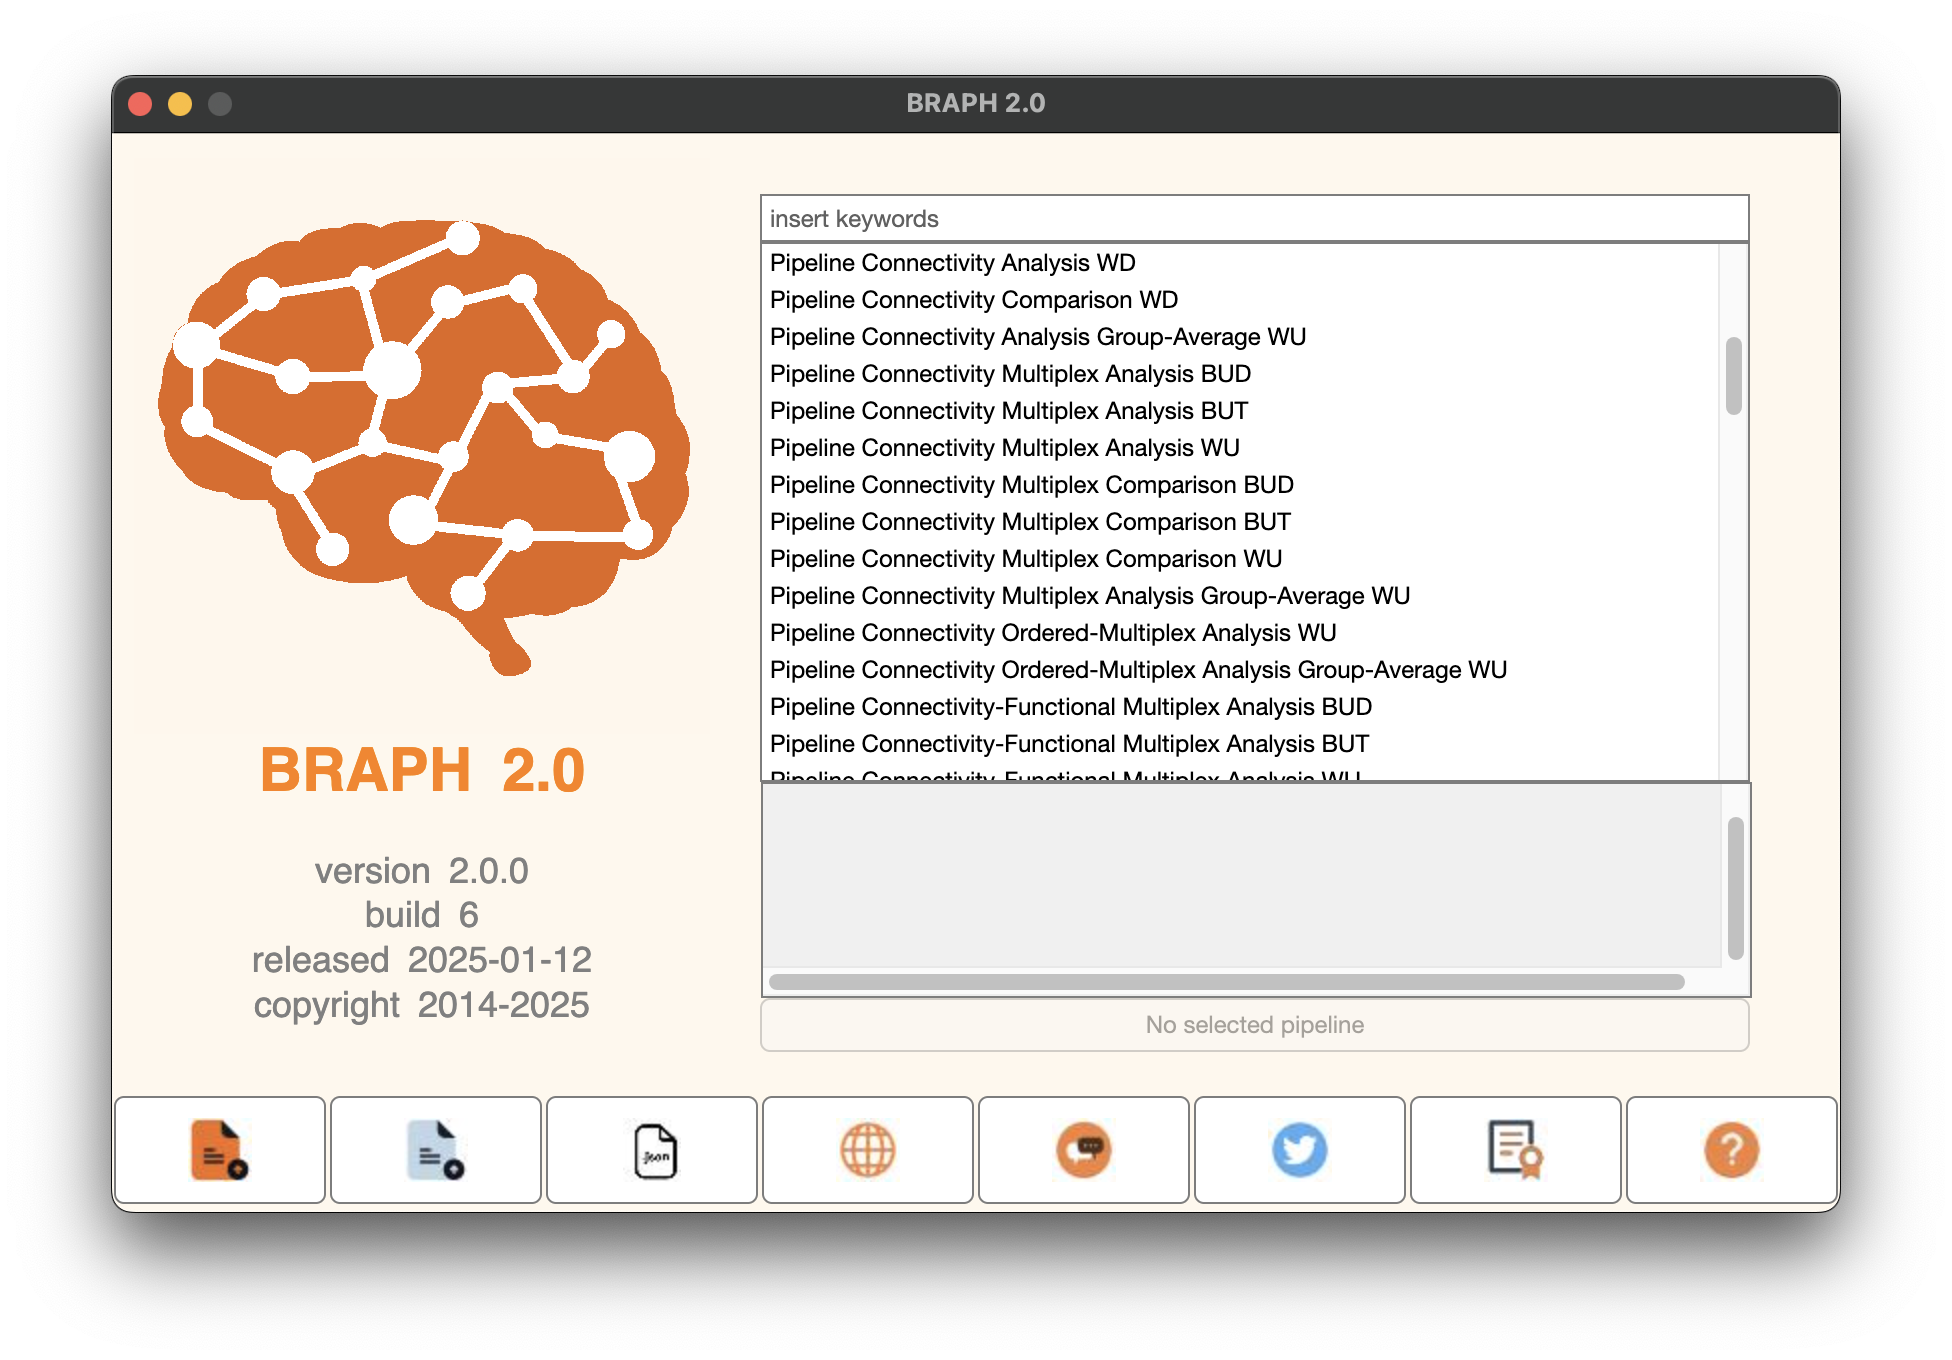
\includegraphics{fig01.png}
}
{BRAPH~2 main GUI}
{
	The BRAPH~2 main GUI displaying a range of pipeline categories, with \textit{Pipeline Comparison Connectivity BUT} selected. You can access the user tutorial for the selected pipeline directly via the context menu by right-clicking on the pipeline and selecting either \textit{Web Tutorial} or \textit{PDF Tutorial}, as shown in \Figref{fig:02}.
}

\fig{marginfigure}
{fig:02}
{
	
\includegraphics{fig02a.png}
	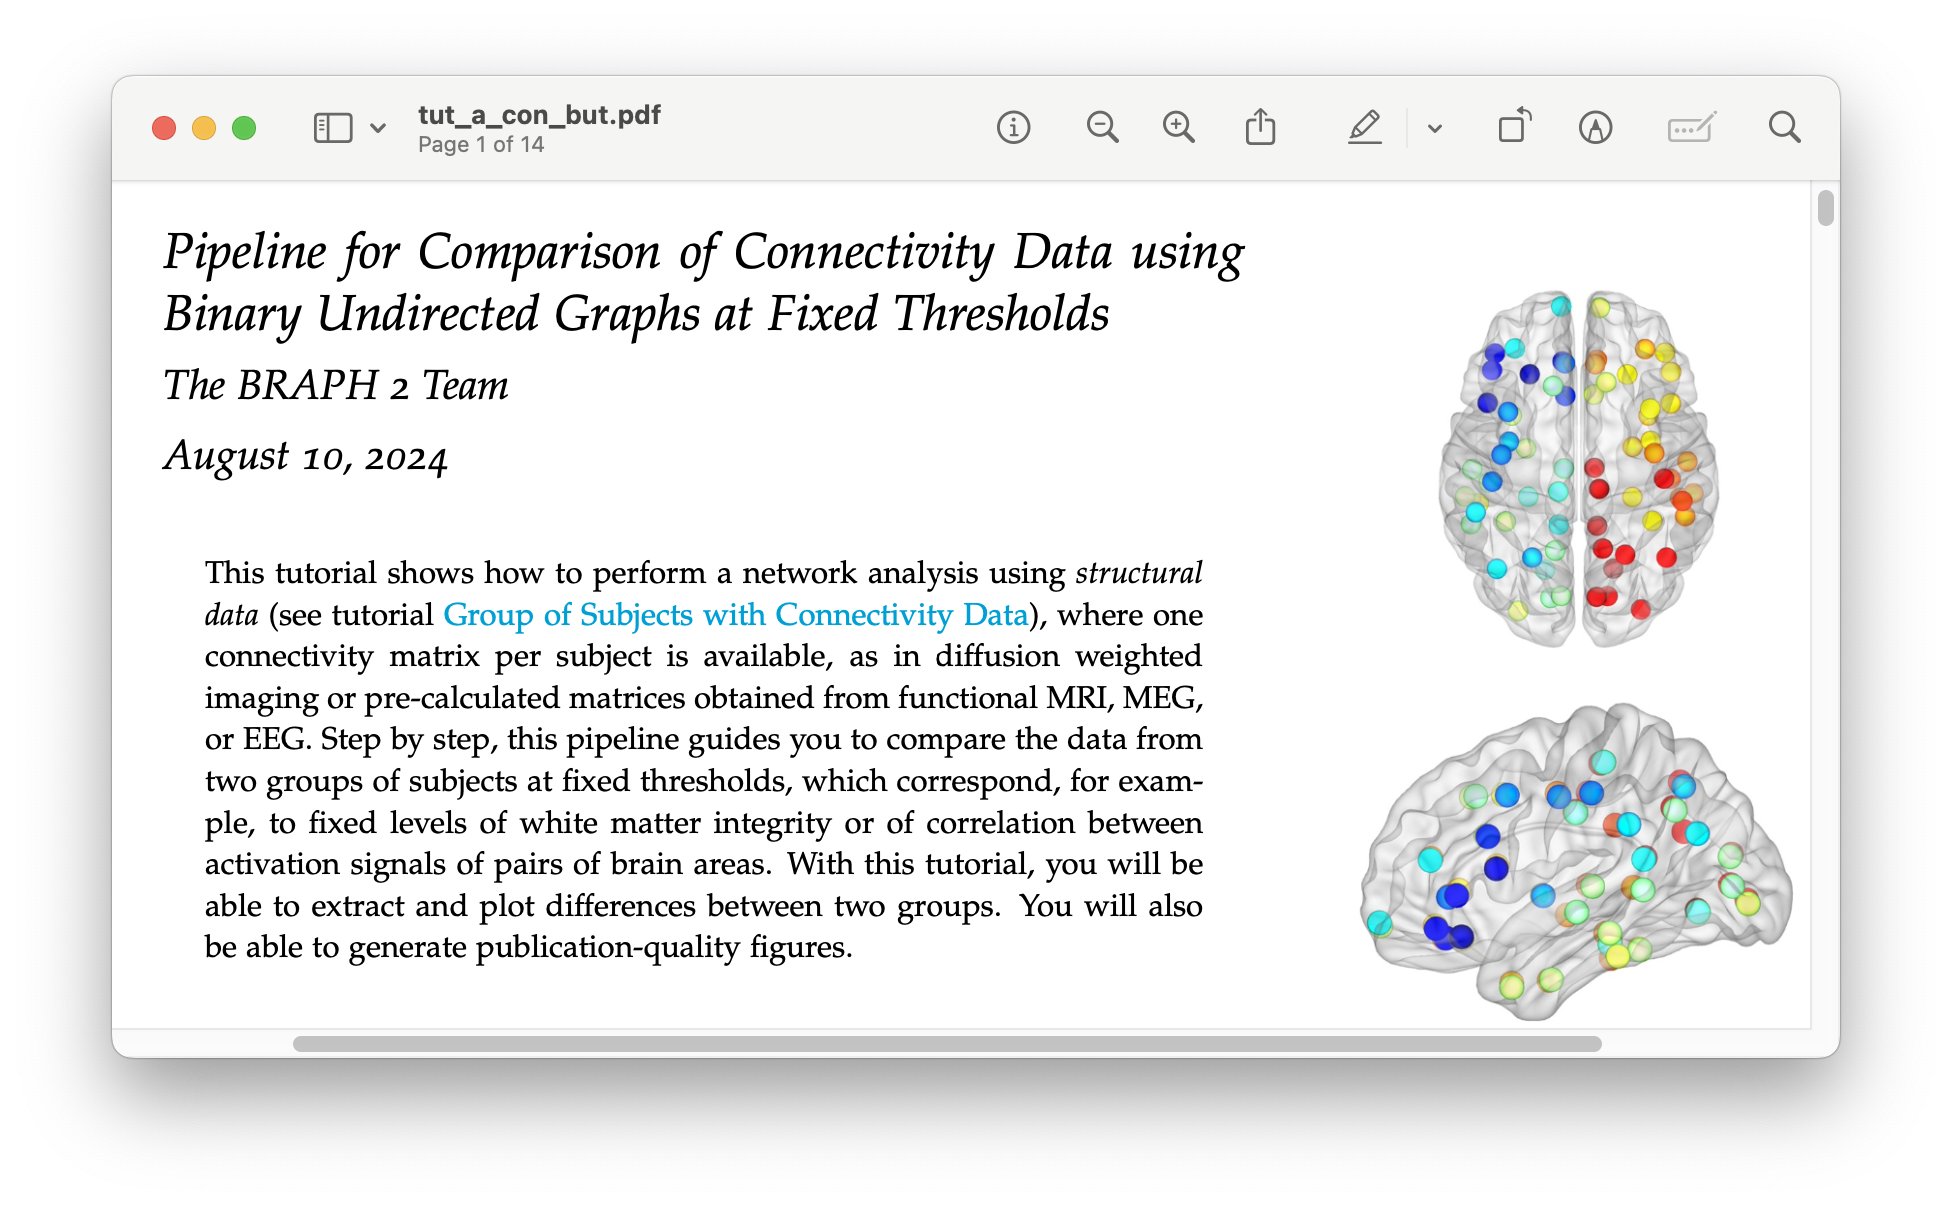
\includegraphics{fig02b.png}
}
{User tutorial for the pipeline}
{
	BRAPH~2 user tutorials accessible either via a browser for its ReadMe version or through a PDF reader for its PDF version. Tutorials for the selected pipeline can be directly accessed from the context menu, as shown in \Figref{fig:01} and \Figref{fig:02}.
}

\subsection{Pipeline Steps}

Each pipeline consists of a series of sequential steps to guide your analysis. For example, a typical graph analysis pipeline might include the following steps:
\begin{enumerate}

\item \textbf{Load Atlas}: Import or select a brain atlas (ROI definitions).

\item \textbf{Load Group(s)}: Load subjects' data (structural, functional, or connectivity matrices).

\item \textbf{Analyze}: Build graphs (optionally threshold them) and compute graph measures.

\item \textbf{Compare (optional)}: If you have multiple groups, run permutation tests or other statistical comparisons.

\item \textbf{Visualize and Export}: Review measures, visualize results (e.g., brain views, adjacency matrices), and export them.

\end{enumerate}

\section{Basic Tutorial Example}

\subsection{Single-Layer Connectivity Analysis}

\begin{enumerate}

\item \textbf{Run the Connectivity Pipeline}:

In the BRAPH-2 main window, pick a pipeline under the ``Connectivity'' tab (e.g., \textit{Pipeline Comparison Connectivity BUT}, shown in \Figref{fig:03}).

\item \textbf{Load Atlas}:

Choose your brain atlas file (e.g., a \texttt{.xls}, \texttt{.txt}, or provided template).


\item \textbf{Load Groups}:

Import each group of subjects (e.g., controls, patients). Each subject should have a connectivity matrix (WU, BUD, or BUT formats).


\item \textbf{Run the Analysis}:

Select graph measures (e.g., degree, clustering).

Click \texttt{Analyze} to compute measure values per subject and per group.

\fig{marginfigure}
{fig:03}
{
	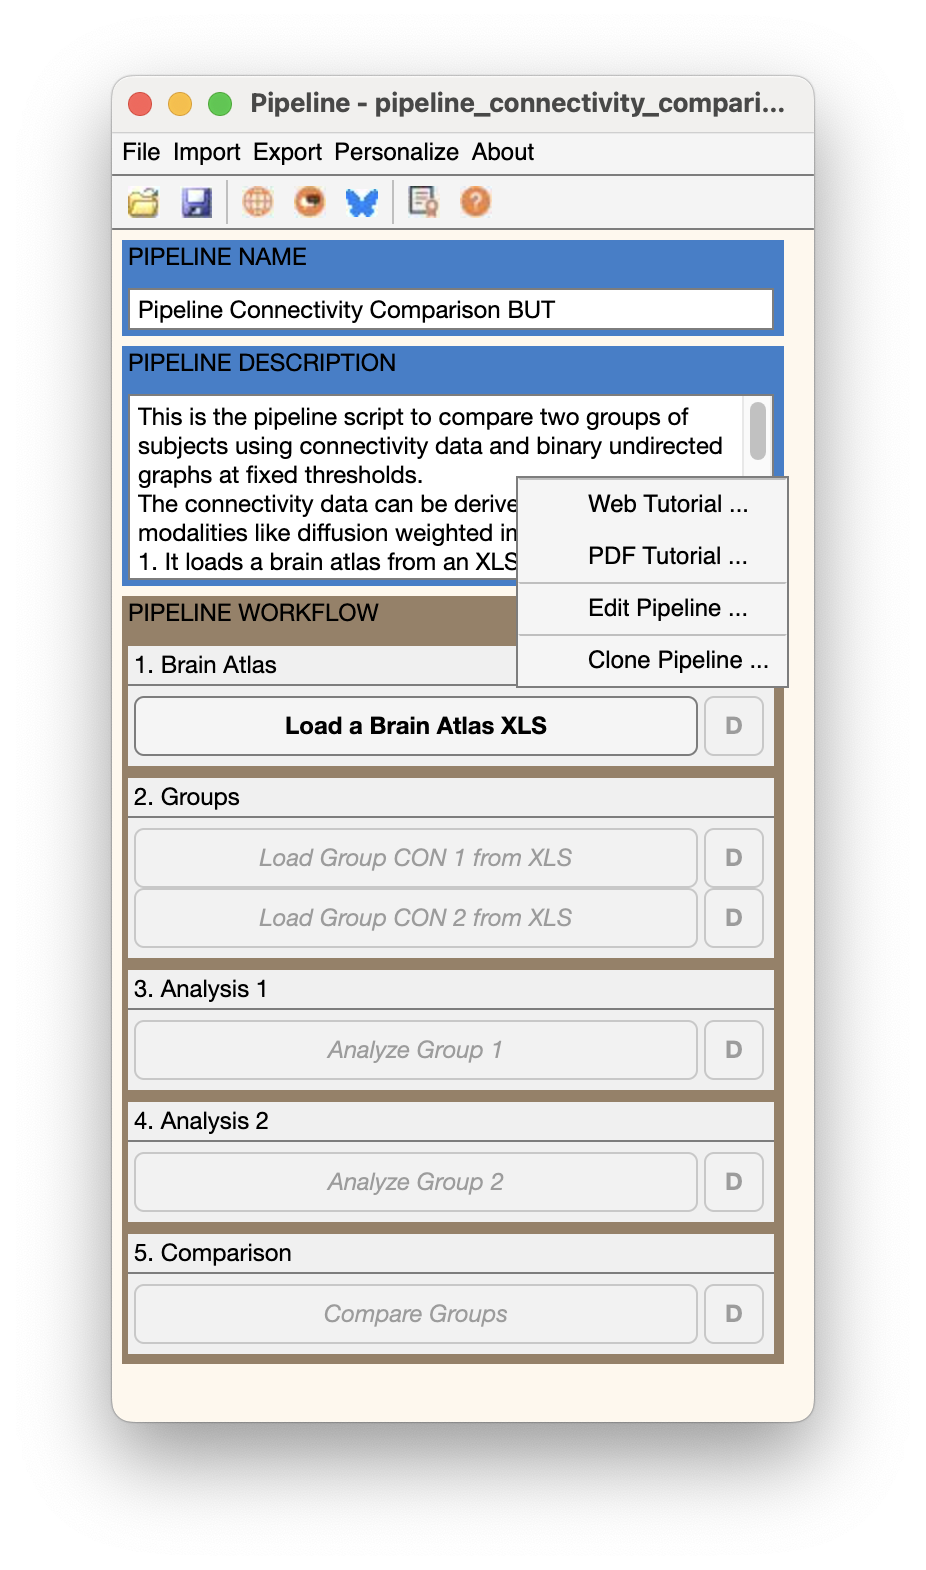
\includegraphics{fig03.png}
}
{Single-layer connectivity analysis}
{
	The \textit{Pipeline Comparison Connectivity BUT} displaying a series of sequential steps for the analysis. You can access the user tutorial for this pipeline directly via the context menu by right-clicking on the pipeline and selecting either \textit{Web Tutorial} or \textit{PDF Tutorial}, as shown in \Figref{fig:02}.
}


\item \textbf{Group Comparison}:

Optionally set up statistical comparisons (e.g., 1000 permutations with FDR correction).

Click \texttt{Compare} to execute.


\item \textbf{Visualize \& Export}:

Examine adjacency matrices, 3D brain plots, bar charts, etc.

Save the pipeline (\texttt{*.b2}), results, and figures for reproducibility.

\end{enumerate}

\subsection{Multilayer and Deep Learning Pipelines}

BRAPH-2 also offers:
\begin{itemize}

\item \textbf{Multilayer Graph Analysis}: Combine multiple modalities (e.g., structural and functional) into a \textit{multiplex} or \textit{multilayer} graph.

\item \textbf{Deep Learning Classification/Regression Pipelines}: Use adjacency matrices or graph measures as input to train neural networks and perform classification (e.g., patient vs. control) or regression (e.g., predict age).

\end{itemize}
These pipelines follow similar steps but involve constructing a \textit{supra-adjacency} matrix (multilayer) or generating input features for neural networks.

\section{Automating Analyses with Scripts}

If you prefer or need batch processing:
\begin{enumerate}

\item Open the \texttt{examples} folder in BRAPH-2 to see sample scripts.

\item Copy and adapt them for your data.  

\item Run in MATLAB to process large datasets or integrate with HPC clusters.

\end{enumerate}

\section{Extending BRAPH-2}

Thanks to its object-oriented architecture:
\begin{itemize}

\item You can create new pipelines by extending existing ones.

\item Add new metrics by subclassing the \texttt{Measure} class.

\item Add new neural network architectures by extending the \texttt{NNBase} class.

\end{itemize}
All changes can be compiled using the command:

\lstinline{braph2genesis}

\section{Further Information}

BRAPH-2 provides a unified environment to explore brain connectivity using modern graph-theoretical methods, multilayer modeling, and deep learning. 
With a simple GUI for non-programmers and rich scripting/development options for advanced users, it accommodates a wide range of neuroscience research needs.

For additional learning resources and reference materials, please see the following.

\subsection{BRAPH-2 GitHub and Discussion Forum}

BRAPH-2 GitHub:

\url{https://github.com/braph-software/BRAPH-2}

\noindent Discussion forum:

\url{https://github.com/braph-software/BRAPH-2/discussions}

\subsection{User Tutorials for Pipelines}

\url{https://github.com/braph-software/BRAPH-2/tree/develop/tutorials/pipelines}

Explore ready-made pipelines for structural, functional, connectivity, and deep learning analyses.

Learn how to load brain atlases, import data, compute graph measures, compare groups, and visualize/export your results.


\subsection{Developer Tutorials for Extending BRAPH-2}

\url{https://github.com/braph-software/BRAPH-2/tree/develop/tutorials/developers}

\textbf{Adapting a Pipeline Script} \url{https://github.com/braph-software/BRAPH-2/tree/develop/tutorials/developers/dev_pipeline}:  
Learn how to modify an existing pipeline, customize parameters (e.g., default number of permutations), or add new pipeline steps.

\textbf{Adapt an Example Script} \url{https://github.com/braph-software/BRAPH-2/tree/develop/tutorials/developers/dev_script}:  
See how to turn a GUI-based analysis into an automated script for batch processing or cluster/HPC applications.

\textbf{Implement, Import, and Export Groups of Subjects} \url{https://github.com/braph-software/BRAPH-2/tree/develop/tutorials/developers/dev_subject}:  
Discover how to introduce new Subject types (e.g., new data modalities), handle group-level imports, and export results.

\textbf{Implement a New Ensemble Analysis} \url{https://github.com/braph-software/BRAPH-2/tree/develop/tutorials/developers/dev_analysis_ensemble}:  
Create advanced ensemble analyses in which a measure is calculated for each subject, enabling subject-level comparisons.

\textbf{Implement a New Group Analysis} \url{https://github.com/braph-software/BRAPH-2/tree/develop/tutorials/developers/dev_analysis_group}:  
Create analyses where measures are computed at the group level (useful for structural pipelines and group-average connectivity).

Implementing new graphs and measures:

\textbf{Implement a New Graph} \url{https://github.com/braph-software/BRAPH-2/tree/develop/tutorials/developers/dev_graph}:  
Learn the steps to create and register novel graph types (e.g., new adjacency representations, directed/undirected, multiplex).

\textbf{Implement a New Measure} \url{https://github.com/braph-software/BRAPH-2/tree/develop/tutorials/developers/dev_measure}:
Extend BRAPH-2 with original graph-theoretical metrics (e.g., community detection, centrality, resilience) by defining measure properties and calculations.

Deep learning tutorials:

\textbf{Implement a New Neural Network Classifier} \url{https://github.com/braph-software/BRAPH-2/tree/develop/tutorials/developers/dev_neural_networks/dev_nn_classifier}:
Build custom classification architectures, integrating them directly into the BRAPH-2 pipelines.

\textbf{Implement a New Neural Network Regressor} \url{https://github.com/braph-software/BRAPH-2/tree/develop/tutorials/developers/dev_neural_networks/dev_nn_regressor}:  
Add regression pipelines for tasks such as age prediction or continuous clinical measures.

\end{document}